\documentclass{beamer}

\mode<presentation>
{
  \usetheme{CambridgeUS}
  \setbeamercovered{transparent}
}

\usepackage[english]{babel}
\usepackage[latin1]{inputenc}
\usepackage{times}
\usepackage[T1]{fontenc} 
% Or whatever. Note that the encoding and the font should match. If T1
% does not look nice, try deleting the line with the fontenc.
\usepackage{amsmath}

\newcommand{\linespace}{\vskip 0.25cm}

\definecolor{MyForestGreen}{rgb}{0,0.7,0} 
\newcommand{\tableemph}[1]{{#1}}
\newcommand{\tablewin}[1]{\tableemph{#1}}
\newcommand{\tablemid}[1]{\tableemph{#1}}
\newcommand{\tablelose}[1]{\tableemph{#1}}

\definecolor{MyLightGray}{rgb}{0.6,0.6,0.6}
\newcommand{\tabletie}[1]{\color{MyLightGray} {#1}}

% The text in square brackets is the short version of your title and will be used in the
% header/footer depending on your theme.
\title[Mobile Security]{Improving Mobile Security}

% Sub-titles are optional - uncomment and edit the next line if you want one.
% \subtitle{Why does sub-tree crossover work?} 

% The text in square brackets is the short version of your name(s) and will be used in the
% header/footer depending on your theme.
\author[Luthi]{Braden Luthi}

% The text in square brackets is the short version of your institution and will be used in the
% header/footer depending on your theme.
\institute[U of Minn, Morris]
{
  Division of Science and Mathematics \\
  University of Minnesota, Morris \\
  Morris, Minnesota, USA
}

% The text in square brackets is the short version of the date if you need that.
\date[April '14, ] % (optional)
{29 April 2014 }

% Delete this, if you do not want the table of contents to pop up at
% the beginning of each subsection:
\AtBeginSection[]
{
  \begin{frame}<beamer>
    \frametitle{Outline}
    \tableofcontents[currentsection, hideothersubsections]
  \end{frame}
}

\begin{document}

\begin{frame}
  \titlepage
\end{frame}

% For a 20-25 minute senior seminar talk you probably want something like:
% - Two or three major sections (other than the summary).
% - At *most* three subsections per section.
% - Talk about 30s to 2min per frame. So there should probably be between
%   15 and 30 frames, all told.

\section*{Overview}


\subsection*{Outline}

\begin{frame}
  \frametitle{Outline}
  \tableofcontents[hideallsubsections]
\end{frame}
\section{Background}
\subsection{GSM and UMTS}
	\subsubsection{GSM}
	\subsubsection{UMTS}
\subsection{Cryptography}
	%basic introduction to cryptography and vocabulary
	%toy cipher example.
\section{GSM Weakness in UMTS}
\subsection{Authentication}
\begin{frame}
% add hidden frames, introduce requests one at a time
  \frametitle{GSM Authentication}
  \begin{center}
  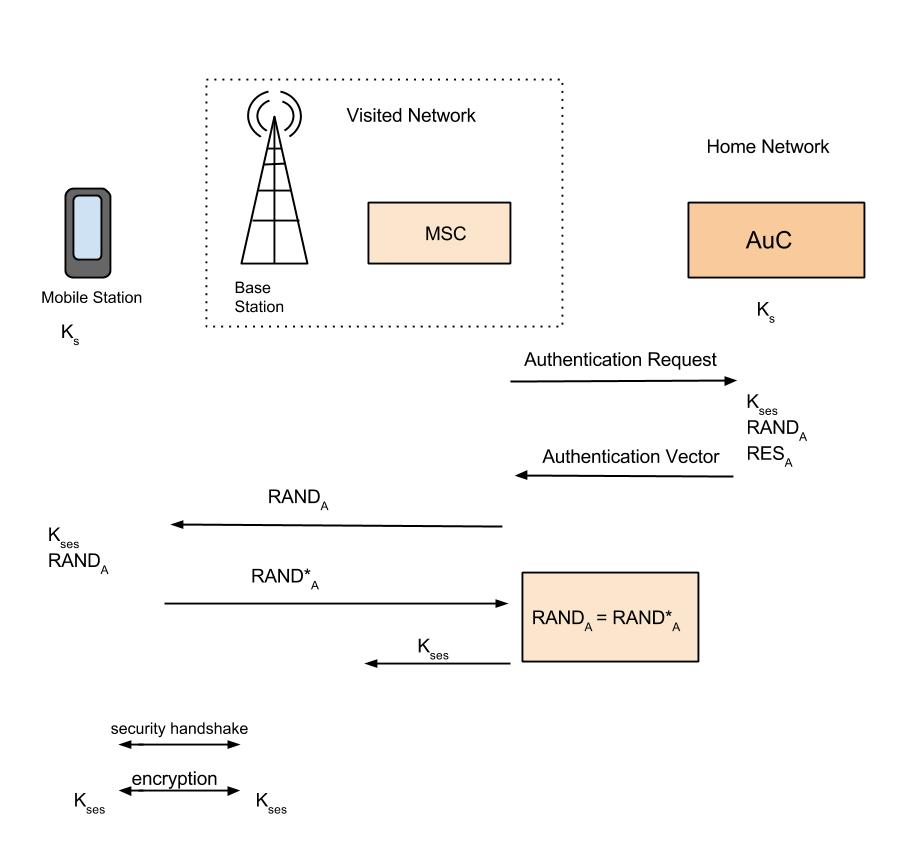
\includegraphics[scale =.25]{GSM Authentication.jpg}

  \end{center} 
\end{frame}

\subsection{GSM and UMTS Inter-working Networks}
\begin{frame}
	\frametitle{Inter-working Networks}
\end{frame}
\subsection{Man-In-The-Middle Attack}
\begin{frame}
	\frametitle{Man-in-the-middle weakness in GSM}
	% refer back to GSM authentication diagram ?
\end{frame}
\subsection{Solution}
\begin{frame}
\frametitle{Protecting UMTS from GSM Man-in-the-middle attack}
\end{frame}
\section{Application Security Threat}
\section{EM Leaking Key Information?}
	\subsection{Side channel attack}
	\subsection{Side channel through EM }

\end{document}


